\documentclass[12pt, letterpaper]{article}
% \documentclass{book}
\title{My first LaTeX document}
\author{Hubert Farnsworth\thanks{Funded by the Overleaf team.}}
\date{August 2022}
\usepackage{graphicx} % LaTeX package to import graphics
\usepackage{amsmath}% For the equation* environment
\graphicspath{{images/}} % configuring the graphicx package

\begin{document}

\maketitle
\begin{abstract}
This is a simple paragraph at the beginning of the 
document. A brief introduction about the main subject.
\end{abstract}

\section{StaUp}
% how a new paragraph is created by pressing the "enter" key twice
After our abstract we can begin the first paragraph, then press ``enter'' twice to start the second one.

This line will start a second paragraph.

% alternatively, use the \newline command.
I will start the third paragraph and then add \\ 
a manual line break which \newline causes this text to start on a new line but remains part of the same paragraph. Alternatively, I can use the \verb|\newline|\newline command to start a new line, which is also part of the same paragraph.


\section{preamble}
We have now added a title, author and date to our first \LaTeX{} document!
The universe is immense and it seems to be homogeneous, 
on a large scale, everywhere we look.\\



\section{How to include pic?}
% The \includegraphics command is 
% provided (implemented) by the 
% graphicx package

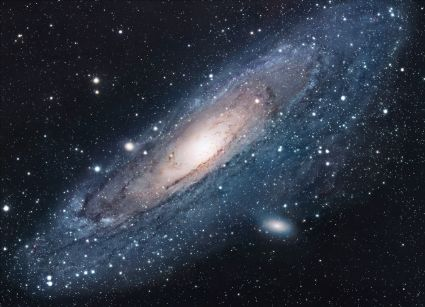
\includegraphics{universe}


There's a picture of a galaxy above.

\begin{figure}[h]
    \centering
    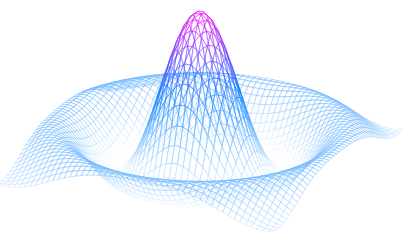
\includegraphics[width=0.75\textwidth]{mesh}
    \caption{a nice plot.}
    \label{fig:mesh1}
\end{figure}
As you can see in figure \ref{fig:mesh1}, the function grows near the origin. This example is on page \pageref{fig:mesh1}.

\begin{itemize}
    \item This is 
    \item 
    \item a
    \item unordered list?
\end{itemize}

\begin{enumerate}
    \item This is 
    \item a
    \item ordered list?
    \item 
\end{enumerate}

\section{type Math formula}

In physics, the mass-energy equivalence is stated 
by the equation $E=mc^2$, discovered in 1905 by Albert Einstein.    

% to typeset display-mode math you should use delimiter pairs
% Historically, typesetting display-mode math required use of $$ characters delimiters, as in $$ ... display math here ...$$, but this method is no longer recommended: use LaTeX’s delimiters \[ ... \] instead.

The mass-energy equivalence is described by the famous equation
\[ E=mc^2 \] discovered in 1905 by Albert Einstein. 

In natural units ($c = 1$), the formula expresses the identity(恒等式)
\begin{equation}
E=mc^2
\end{equation}
or in this way
\begin{displaymath}
E=mc^2
\end{displaymath}

Subscripts in math mode are written as $a_b$ and superscripts are written as $a^b$. These can be combined and nested to write expressions such as

\[ T^{i_1 i_2 \dots i_p}_{j_1 j_2 \dots j_q} = T(x^{i_1},\dots,x^{i_p},e_{j_1},\dots,e_{j_q}) \]
We write integrals using $\int$ and fractions using $\frac{a}{b}$. Limits are placed on integrals using superscripts and subscripts:

\[ \int_0^1 \frac{dx}{e^x} =  \frac{e-1}{e} \]

Lower case Greek letters are written as $\omega$ $\delta$ etc. while upper case Greek letters are written as $\Omega$ $\Delta$.

Mathematical operators are prefixed with a backslash as $\sin(\beta)$, $\cos(\alpha)$, $\log(x)$ etc.

\section{First example - mutiple-line formula}

The well-known Pythagorean theorem\text{毕达哥拉斯定理} \(x^2 + y^2 = z^2\) was proved to be invalid for other exponents, meaning the next equation has no integer solutions for \(n>2\):

\[ x^n + y^n = z^n \]

\section*{Second example - mutiple-line formula}

This is a simple math expression \(\sqrt{x^2+1}\) inside text. 
And this is also the same: 
\begin{math}
    \sqrt{x^2+1}
\end{math}
but by using another command.

This is a simple math expression without numbering
\[\sqrt{x^2+1}\] 
separated from text.

This is also the same:
\begin{displaymath}
    \sqrt{x^2+1}
\end{displaymath}

\ldots and this:
\begin{equation*}
    \sqrt{x^2+1}
\end{equation*}


\section*{Second example - mutiple-line formula}

\begin{center}
    \begin{tabular}{c c c}
        cell1 & cell2 & cell3 \\ 
        cell4 & cell5 & cell6 \\  
        cell7 & cell8 & cell9    
    \end{tabular}
    \begin{tabular}{|c|c|c|} 
        \hline
        cell1 & cell2 & cell3 \\ 
        cell4 & cell5 & cell6 \\ 
        cell7 & cell8 & cell9 \\ 
        \hline
    \end{tabular}

\end{center}

\begin{center}
    \begin{tabular}{||c c c c||} 
    \hline
    Col1 & Col2 & Col2 & Col3 \\ [0.5ex] 
    \hline\hline
    1 & 6 & 87837 & 787 \\ 
    \hline
    2 & 7 & 78 & 5415 \\
    \hline
    3 & 545 & 778 & 7507 \\
    \hline
    4 & 545 & 18744 & 7560 \\
    \hline
    5 & 88 & 788 & 6344 \\ [1ex] 
    \hline
    \end{tabular}
\end{center}

Table \ref{table:data} shows how to add a table caption and reference a table.
\begin{table}[h!]
    \centering
    \begin{tabular}{||c c c c||} 
    \hline
    Col1 & Col2 & Col2 & Col3 \\ [0.5ex] 
    \hline\hline
    1 & 6 & 87837 & 787 \\ 
    2 & 7 & 78 & 5415 \\
    3 & 545 & 778 & 7507 \\
    4 & 545 & 18744 & 7560 \\
    5 & 88 & 788 & 6344 \\ [1ex] 
    \hline
    \end{tabular}
    \caption{Table to test captions and labels.}
\label{table:data}
\end{table}

\end{document}

